\documentclass[12pt]{article}

\usepackage{scicite,times,graphicx,float,hyperref}
\usepackage[skip=0pt]{caption}
\usepackage[utf8]{inputenc}
\usepackage{enumitem}
\usepackage{booktabs}

\topmargin -1.0cm
\oddsidemargin 0.0cm
\textwidth 16cm 
\textheight 23cm
\footskip 1.0cm

\newenvironment{sciabstract}{%
\begin{quote} \bf}
{\end{quote}}

\newcounter{lastnote}
\newenvironment{scilastnote}{%
  \setcounter{lastnote}{\value{enumiv}}%
  \addtocounter{lastnote}{+1}%
  \begin{list}%
  {\arabic{lastnote}.}
  {\setlength{\leftmargin}{.22in}}
  {\setlength{\labelsep}{.5em}}
}
{\end{list}}

\title{A Kafka-Based Centralized Platform\\for Smart Vehicle Supervising} 

\author
{Filipe Pires [85122], João Alegria [85048]\\
\\
Software Architecture\\
\normalsize{Department of Electronics, Telecommunications and Informatics}\\
\normalsize{University of Aveiro}\\
} 

\date{\today{}}

%%%%%%%%%%%%%%%%% END OF PREAMBLE %%%%%%%%%%%%%%%%

\begin{document} 

\baselineskip18pt

\maketitle 

\section{Introduction} %%%%%%%%%%%%%%%%%%%%%%%%%%%%%%%%%%%%%%%%%%%%%%%%%%%%%%%%%%%%%%%%%%%%%%%%%%%%%%%%%%%%%%%%%%%%%%%%%%%%%%%%%%%%%%%%%%%%%%%%%%%%%%%%%%%%%%%%%

This report aims to describe the work developed for the second assignment of the course of 'Software Architecture', focused on a platform that collects and 
processes information from simulated vehicles.

....................

We also mention how the work was distributed amongst the authors.
All code developed is publicly accessible in our GitHub repository:
\url{https://github.com/FilipePires98/AS/}.
\newpage

\section{.........} %%%%%%%%%%%%%%%%%%%%%%%%%%%%%%%%%%%%%%%%%%%%%%%%%%%%%%%%%%%%%%%%%%%%%%%%%%%%%%%%%%%%%%%%%%%%%%%%%%%%%%%%%%%%%%%%%%%%%%%%%%%%%%%%%%%%%%%%%%%%

.......................

\subsection{.........} %%%%%%%%%%%%%%%%%%%%%%%%%%%%%%%%%%%%%%%%%%%%%%%%%%%%%%%%%%%%%%

......................


% \vspace{-10pt}
% \begin{itemize}[noitemsep]
%   \item Prepare - the selected farmers move to a Standing Area, ready for orders.
%   \item Start - the actual simulation begins and farmers start moving.
%   \item Collect - farmers collect corn cobs from the Granary (where the cobs initially are).
%   \item Return - farmers return to the Storehouse with the collected corn cobs.
%   \item Stop - farmers stop whatever they are doing and return to the Storehouse.
%   \item Exit - simulation ends and the program closes.
% \end{itemize}
% \vspace{-10pt}

% \begin{figure}[H]
%   \centering
%   \begin{minipage}{\textwidth}
%     \centering
%     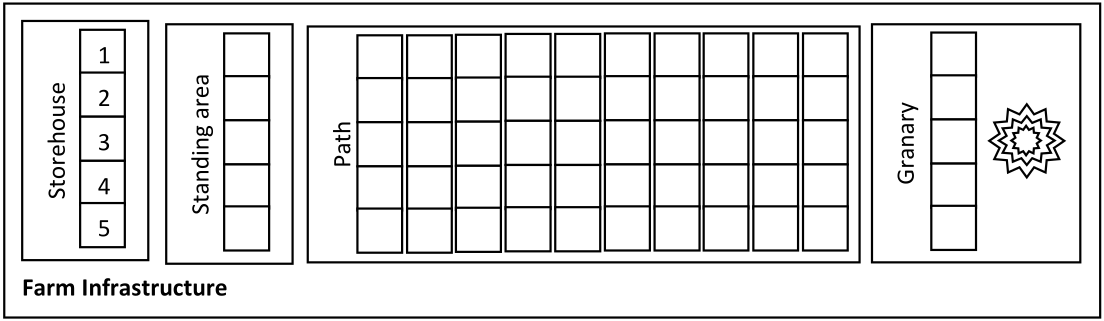
\includegraphics[width=\linewidth]{img/Design_FI.png}
%   \end{minipage}%
%   \caption{Visual representation of the farm, taken from \cite{assign}.}
%   \label{Design_FI}
% \end{figure} 

%\texttt{java -cp <userdir>/build/classes fi.FarmInfrastructure}

\section{............} %%%%%%%%%%%%%%%%%%%%%%%%%%%%%%%%%%%%%%%%%%%%%%%%%%%%%%%%%%%%%%%%%%%%%%%%%%%%%%%%%%%%%%%%%%%%%%%%%%%%%%%%%%%%%%%%%%%%%%%%%%%%%%%%%%

.........................

\section{Additional Remarks} %%%%%%%%%%%%%%%%%%%%%%%%%%%%%%%%%%%%%%%%%%%%%%%%%%%%%%%%%%%%%%%%%%%%%%%%%%%%%%%%%%%%%%%%%%%%%%%%%%%%%%%%%%%%%%%%%%%%%%%%%%%%%%%%%%%

\subsection{Documentation} %%%%%%%%%%%%%%%%%%%%%%%%%%%%%%%%%

...................

\subsection{Assignment Contributions} %%%%%%%%%%%%%%%%%%%%%%

...................

\section{Conclusions} %%%%%%%%%%%%%%%%%%%%%%%%%%%%%%%%%%%%%%%%%%%%%%%%%%%%%%%%%%%%%%%%%%%%%%%%%%%%%%%%%%%%%%%%%%%%%%%%%%%%%%%%%%%%%%%%%%%%%%%%%%%%%%%%%%%%%%%%%%

........................

\begin{thebibliography}{9} %%%%%%%%%%%%%%%%%%%%%%%%%%%%%%%%%%%%%%%%%%%%%%%%%%%%%%%%%%%%%%%%%%%%%%%%%%%%%%%%%%%%%%%%%%%%%%%%%%%%%%%%%%%%%%%%%%%%%%%%%%%%%%%%%%%%%
  \bibliographystyle{Science}

  \bibitem{assign}
    Óscar Pereira,
    \textit{SA: Practical Assignment no.2},
    University of Aveiro,
    2019/20.

  % \bibitem{uml}
  %   Object Management Group,
  %   \textit{What is UML},
  %   \url{https://www.uml.org/what-is-uml.htm},
  %   accessed in March 2020.
    
  % \bibitem{javadoc}
  %   Oracle,
  %   \textit{Javadoc Technology},
  %   \url{https://docs.oracle.com/javase/8/docs/technotes/guides/javadoc/index.html},
  %   accessed in February 2020.

\end{thebibliography}

\clearpage

\end{document}




















